
%(BEGIN_QUESTION)
% Copyright 2011, Tony R. Kuphaldt, released under the Creative Commons Attribution License (v 1.0)
% This means you may do almost anything with this work of mine, so long as you give me proper credit

Calculate the reset time period of this integral-only controller, its output signal given the following conditions, and also its direction of action:

$$\includegraphics[width=15.5cm]{i00809x01.eps}$$

Reset time = \underbar{\hskip 50pt} minutes per repeat

\vskip 10pt

\noindent
Supposing:

\begin{itemize}
\item{} SP signal = 3 volts (constant)
\item{} PV signal = 2.4 volts (constant)
\item{} Output signal (at time = 0) = 3.4 volts
\end{itemize}

\vskip 10pt

Output signal (at time = 3.3 minutes) = \underbar{\hskip 50pt} volts

\vskip 10pt

{\it Direct} or {\it Reverse} action?

\underbar{file i00809}
%(END_QUESTION)





%(BEGIN_ANSWER)

I recommend 3 points for proper reset time, 4 points for output signal calculation, and 3 points for proper action:

\vskip 10pt

Reset time = \underbar{\bf 1.485} minutes per repeat

\vskip 10pt

Output signal (at time = 3.3 minutes) = \underbar{\bf 4.733} volts

\vskip 10pt

{\bf Reverse} action

%(END_ANSWER)





%(BEGIN_NOTES)

{\bf This question is intended for exams only and not worksheets!}.

%(END_NOTES)


